\section{Performance Tuning}
\label{section:performance}


\subsection{Non-bonded interaction distance-testing}

The last critical parameter for non-bonded
interaction calculations is the parameter {\tt pairlistdist}.  To reduce the
cost of performing the non-bonded interactions, \NAMD\ uses a {\it non-bonded
pair list} which contained all pairs of atoms for which
non-bonded interactions
should be calculated.  Performing the search for pairs of atoms that
should have their interactions calculated is an expensive operation.  Thus,
the pair list is only calculated periodically, at least once per cycle.
Unfortunately,
pairs of atoms move relative to each other during the steps between preparation
of the pair list.  Because of this, if the pair list were built to include
only
those pairs of atoms that are within the cutoff distance
when the list is generated, it would
be possible 
for atoms to drift closer together
than the cutoff distance during subsequent timesteps and yet not
have their non-bonded interactions calculated.  
\prettypar
Let us consider a concrete example to better understand this.  Assume that the
pairlist is built once every ten timesteps and that the cutoff
distance is 8.0 \AA.  Consider a pair
of atoms A and B that are 8.1 \AA\ apart when the pairlist is built.
If the pair list
includes only those atoms within the cutoff distance, this pair would not
be included in the list.  Now assume that after five timesteps, atoms
A and B have moved to only 7.9 \AA\ apart.  A and B are now within the
cutoff distance of each other, and should have their
non-bonded interactions calculated.
However, because the non-bonded interactions are based solely on the pair list
and the pair list will not be rebuilt for another five timesteps, this pair
will be ignored for five timesteps causing energy not to be conserved 
within the system.  
\prettypar
To avoid this problem, the parameter {\tt pairlistdist} allows the user
to specify a distance greater than the {\tt cutoff} distance for pairs
to be included in the pair list, as shown in Figure \ref{fig:pairlistdist}.
Pairs that are included in the pair list but are outside the cutoff distance
are simply ignored.  So in the above example, if the {\tt pairlistdist}
were set to $10.0$ \AA, then 
the atom pair A and B would be included in the pair list, even though
the pair would initially be ignored because they are further apart than
the cutoff distance.  As the pair moved closer and entered the cutoff
distance, because the pair was already in the pair list, the non-bonded
interactions would immediately be calculated and energy conservation
would be preserved.  The value of {\tt pairlistdist} should be chosen
such that no atom pair moves more than 
$\mbox{{\tt pairlistdist}}-\mbox{{\tt cutoff}}$ 
in one cycle.  This will insure energy conservation and efficiency.

\begin{figure}[htb]
  \center{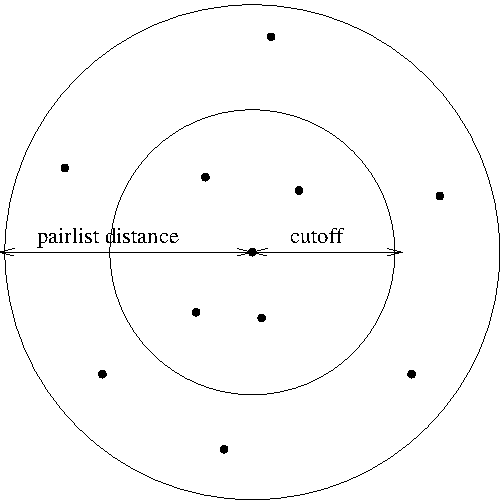
\includegraphics{figures/pairlistdist}}
  \caption[Example of cutoff and pairlist distance uses]
  {{\small Depiction of the difference between the cutoff distance and the
  pair list distance.  The pair list distance specifies a sphere that is
  slightly larger than that of the cutoff so that pairs are allowed to
  move in and out of the cutoff distance without causing energy conservation
  to be disturbed.}}
  \label{fig:pairlistdist}
\end{figure}

The {\tt pairlistdist} parameter is also used to determine the minimum patch size.
Unless the {\tt splitPatch} parameter is explicitly set to {\tt position}, hydrogen atoms will be placed on the same patch as the ``mother atom'' to which they are bonded.
These {\em hydrogen groups} are then distance tested against each other using only a cutoff increased by the the value of the {\tt hgroupCutoff} parameter.
The size of the patches is also increased by this amount.
\NAMD\ functions correctly even if a hydrogen atom and its mother atom are separated by more than half of {\tt hgroupCutoff} by breaking that group into its individual atoms for distance testing.
Margin violation warning messages are printed if an atom moves outside of a safe zone surrounding the patch to which it is assigned, indicating that {\tt pairlistdist} should be increased in order for forces to be calculated correctly and energy to be conserved.

\index{margin violations}
Margin violations mean that atoms that are in non-neighboring patches may
be closer than the cutoff distance apart.  This may sometimes happen in
constant pressure simulations when the cell shrinks (since the patch grid
remains the same size).  The workaround is to increase the margin
parameter so that the simulation starts with fewer, larger patches.
Restarting the simulation will also regenerate the patch grid.

In rare special circumstances atoms that are involved in bonded terms
(bonds, angles, dihedrals, or impropers) or nonbonded exclusions (especially
implicit exclusions due to bonds) will be placed on non-neighboring
patches because they are more than the cutoff distance apart.  This can
result in the simulation dying with a message of
``bad global exclusion count''.
\index{Atoms moving too fast}
\index{error message!Atoms moving too fast}
\index{Bad global exclusion count}
\index{error message!Bad global exclusion count}
If an ``atoms moving too fast; simulation has become unstable'',
``bad global exclusion count'', or similar error happens
on the first timestep then there is likely something very
wrong with the input coordinates, such as the atoms with uninitialized
coordinates or different atom orders in the PSF and PDB file.  Looking at
the system in VMD will often reveal an abnormal structure.
Be aware that the atom IDs in the ``Atoms moving too fast'' error
message are 1-based, while VMD's atom indices are 0-based.
If an ``atoms moving too fast; simulation has become unstable'',
``bad global exclusion count'', or similar error happens
later in the simulation then the dynamics have
probably become unstable, resulting in the system ``exploding'' apart.
Energies printed at every timestep should show an exponential increase.
This may be due to a timestep that is too long, or some other strange
feature.  Saving a trajectory of every step and working backwards in
can also sometimes reveal the origin of the instability.


\begin{itemize}

\item
\NAMDCONFWDEF{pairlistdist}
{distance between pairs for inclusion in pair lists (\AA)}
{positive decimal $\geq$ {\tt cutoff}}
{{\tt cutoff}}
{
A pair list is generated {\tt pairlistsPerCycle} times each cycle, 
containing pairs of atoms for which 
electrostatics and van der Waals interactions will be calculated.
This parameter is used when {\tt switching} is set to {\tt on} to
specify the allowable distance between atoms for inclusion in the
pair list.  
This parameter is equivalent to the X-PLOR parameter {\tt CUTNb}.
If no atom moves more than {\tt pairlistdist}$-${\tt cutoff} during
one cycle, then there will be no jump in electrostatic or van der
Waals energies when the next pair list is built.  Since such a jump
is unavoidable when truncation is used, this parameter may only
be specified when {\tt switching} is set to {\tt on}.  If this
parameter is not specified and {\tt switching} is set to {\tt on},
the value of {\tt cutoff} is used.  
A value of at least one greater than {\tt cutoff} is recommended.  
}

\item
\NAMDCONFWDEF{stepspercycle}{timesteps per cycle}{positive integer}{20}
{Number of timesteps in each cycle.  Each cycle represents the number 
of timesteps between atom reassignments.
For more details on non-bonded force evaluation, see
Section \ref{section:electdesc}.}

\item
\NAMDCONFWDEF{splitPatch}
{how to assign atoms to patches}
{{\tt position} or {\tt hydrogen}}
{{\tt hydrogen}}
{
When set to {\tt hydrogen}, hydrogen atoms are kept on the same patch as their parents, allowing faster distance checking and rigid bonds.
}

\item
\NAMDCONFWDEF{hgroupCutoff (\AA)}
{used for group-based distance testing}
{positive decimal}
{2.5}
{
This should be set to twice the largest distance which will ever occur between a hydrogen atom and its mother.  Warnings will be printed if this is not the case.  This value is also added to the margin.
}

\item
\NAMDCONFWDEF{margin}
{extra length in patch dimension (\AA)}{positive decimal}{0.0}
{An internal tuning parameter used in determining the size of the cubes 
of space with which \NAMD\ uses to partition the system.  The value of 
this parameter will not change the physical results of the simulation.  
Unless you are very motivated to get the {\it very} best 
possible performance, just leave this value at the default.}

\item
\NAMDCONFWDEF{pairlistMinProcs}{min procs for pairlists}
{positive integer}{1}
{
Pairlists may consume a large amount of memory as atom counts, densities,
and cutoff distances increase.  Since this data is distributed across
processors it is normally only problematic for small processor counts.
Set pairlistMinProcs to the smallest number of processors on which
the simulation can fit into memory when pairlists are used.
}

\item
\NAMDCONFWDEF{pairlistsPerCycle}{regenerate x times per cycle}
{positive integer}{2}
{
Rather than only regenerating the pairlist at the beginning of a cycle,
regenerate multiple times in order to better balance the costs of
atom migration, pairlist generation, and larger pairlists.
}

\item
\NAMDCONFWDEF{outputPairlists}{how often to print warnings}
{non-negative integer}{0}
{
If an atom moves further than the pairlist tolerance during a simulation
(initially (pairlistdist - cutoff)/2 but refined during the run) any
pairlists covering that atom are invalidated and temporary pairlists
are used until the next full pairlist regeneration.  All interactions
are calculated correctly, but efficiency may be degraded.  Enabling
outputPairlists will summarize these pairlist violation warnings
periodically during the run.
}

\item
\NAMDCONFWDEF{pairlistShrink}{tol *= (1 - x) on regeneration}
{non-negative decimal}{0.01}
{
In order to maintain validity for the pairlist for an entire cycle,
the pairlist tolerance (the distance an atom can move without causing
the pairlist to be invalidated) is adjusted during the simulation.
Every time pairlists are regenerated the tolerance is reduced by
this fraction.
}

\item
\NAMDCONFWDEF{pairlistGrow}{tol *= (1 + x) on trigger}
{non-negative decimal}{0.01}
{
In order to maintain validity for the pairlist for an entire cycle,
the pairlist tolerance (the distance an atom can move without causing
the pairlist to be invalidated) is adjusted during the simulation.
Every time an atom exceeds a trigger criterion that is some fraction
of the tolerance distance, the tolerance is increased by this fraction.
}

\item
\NAMDCONFWDEF{pairlistTrigger}{trigger is atom beyond (1 - x) * tol}
{non-negative decimal}{0.3}
{
The goal of pairlist tolerance adjustment is to make pairlist invalidations
rare while keeping the tolerance as small as possible for best performance.
Rather than monitoring the (very rare) case where atoms actually move more
than the tolerance distance, we reduce the trigger tolerance by this
fraction.  The tolerance is increased whenever the trigger tolerance is
exceeded, as specified by pairlistGrow.
}

\end{itemize}
